\documentclass{article}
\usepackage{graphicx} % 用于插入图片
\usepackage{float}
% if you need to pass options to natbib, use, e.g.:
%     \PassOptionsToPackage{numbers, compress}{natbib}
% before loading neurips_2024

% ready for submission
\usepackage{mathptmx}  % Use Times font for math
\usepackage[numbers]{natbib}
\usepackage{neurips_2024}

\usepackage{xeCJK}     % 支持中文

% 设置中文字体(可以根据需要修改)
\setCJKmainfont{Microsoft YaHei}
\setmainfont{Times New Roman}  % 设置英文字体

% to compile a preprint version, e.g., for submission to arXiv, add add the
% [preprint] option:
%     \usepackage[preprint]{neurips_2024}


% to compile a camera-ready version, add the [final] option, e.g.:
%     \usepackage[final]{neurips_2024}


% to avoid loading the natbib package, add option nonatbib:
%    \usepackage[nonatbib]{neurips_2024}


\usepackage[utf8]{inputenc} % allow utf-8 input
\usepackage[T1]{fontenc}    % use 8-bit T1 fonts
\usepackage{hyperref}       % hyperlinks
\usepackage{url}            % simple URL typesetting
\usepackage{booktabs}       % professional-quality tables
\usepackage{amsfonts}       % blackboard math symbols
\usepackage{nicefrac}       % compact symbols for 1/2, etc.
\usepackage{microtype}      % microtypography
\usepackage{xcolor}         % colors


\title{基于指令微调的数学推理任务探索}


% The \author macro works with any number of authors. There are two commands
% used to separate the names and addresses of multiple authors: \And and \AND.
%
% Using \And between authors leaves it to LaTeX to determine where to break the
% lines. Using \AND forces a line break at that point. So, if LaTeX puts 3 of 4
% authors names on the first line, and the last on the second line, try using
% \AND instead of \And before the third author name.


% \author{%
%   David S.~Hippocampus\thanks{Use footnote for providing further information
%     about author (webpage, alternative address)---\emph{not} for acknowledging
%     funding agencies.} \\
%   Department of Computer Science\\
%   Cranberry-Lemon University\\
%   Pittsburgh, PA 15213 \\
%   \texttt{hippo@cs.cranberry-lemon.edu} \\
%   % examples of more authors
%   \And
%   Coauthor Name \\  % 合作者姓名
%   Department of Mathematics \\  % 合作者所在院系
%   Lemonberry University \\  % 合作者所在大学
%   Pittsburgh, PA 15214 \\  % 合作者所在城市和邮政编码
%   \texttt{coauthor@lemonberry.edu} % 合作者电子邮件
%   % \And
%   % Coauthor \\
%   % Affiliation \\
%   % Address \\
%   % \texttt{email} \\
%   % \AND
%   % Coauthor \\
%   % Affiliation \\
%   % Address \\
%   % \texttt{email} \\
%   % \And
%   % Coauthor \\
%   % Affiliation \\
%   % Address \\
%   % \texttt{email} \\
%   % \And
%   % Coauthor \\
%   % Affiliation \\
%   % Address \\
%   % \texttt{email} \\
% }


\author{
    Huazheng~Zeng\\
    School of Computer Science and Technology \\
    Fudan University \\
    220 Handan Rd, Shanghai \\
    \texttt{22302010022@m.fudan.edu} \\
    \AND
    Yang~Wang\\
    School of Computer Science and Technology \\
    Fudan University \\
    220 Handan Rd, Shanghai \\
    \texttt{22302010020@m.fudan.edu} \\
    \AND
    Yuxuan~Xie\\
    School of Computer Science and Technology \\
    Fudan University \\
    220 Handan Rd, Shanghai \\
    \texttt{22302010066@m.fudan.edu} \\
    % Coauthor Name \\
    % Department of Mathematics \\
    % Lemonberry University \\
    % Pittsburgh, PA 15214 \\
    % \texttt{coauthor@lemonberry.edu} \\
    % \And
    % Another Coauthor Name \\
    % Department of Physics \\
    % Raspberry College \\
    % Pittsburgh, PA 15215 \\
    % \texttt{another@raspberry.edu}
}


\begin{document}


\maketitle


\begin{abstract}
  数学推理是评估人类智力基本认知能力的基石。近年来,针对自动解决数学问题的大型语言模型LLMs得到了显著发展。
  我们基于Qwen2.5-0.5B-instruction,探索了全参数SFT,全参数LoRA指令微调的效果,
  同时,通过数据集增强,提高了模型的性能;我们还在解码阶段加入多轮投票,得到了相关的测试结果。
\end{abstract}



\section{Introduction}

数学推理是评估人类智力的核心任务之一。随着大规模语言模型(LLMs)的不断发展,基于自然语言处理的数学推理任务已成为一个重要的研究领域。尽管传统的数学推理方法依赖于符号计算和规则推导,近年来,深度学习,尤其是大型语言模型,已经在自动推理方面取得了显著的进展。

本研究基于Qwen2.5-0.5B-instruction模型,探讨了指令微调(instruction fine-tuning)方法在数学推理任务中的应用,重点研究了全参数微调(SFT)和LoRA微调两种技术的效果。此外,我们还结合了数据增强策略,通过DeepSeek API扩展训练数据集,以提升模型在复杂数学推理任务中的表现。为进一步增强模型的推理能力,我们在解码阶段引入了多轮投票机制,旨在通过集成多次推理结果来提高推理的稳定性和准确性。

本文的主要贡献包括:提出了Qwen2.5模型在数学推理任务中的应用,探索了不同微调技术的效果,并评估了数据增强和投票机制在该任务中的有效性。







\section{RelatedWork}

\subsection{大语言模型的能力与优化}
大语言模型(LLMs)在自然语言处理(NLP)任务中展现了革命性能力。QWEN\cite{bai2023qwentech},GPT-4通过指令微调开发了面向特定领域的专精模型。其架构结合多参数规模的基础模型和对话模型,通过强化学习与人类反馈调节技术(RLHF)进一步优化,展现出卓越的适应性与问题解决能力\cite{bai2023qwentech}\cite{openai2024gpt4}。

\subsection{数学推理领域的研究进展}
数学推理领域的研究历程从符号计算与公式解析发展到基于深度学习的自动化方法。QWEN在精细预训练和微调策略的支持下,显著提升了复杂推理路径与工具使用的能力,结合提示工程进一步优化了其在数学推理任务中的表现。现有研究中,基于单一模型的微调方法在扩展性和泛化能力上存在一定局限性。例如,Janice Ahn 等人采纳包含 Q-A、Question-Equation-Answer 和 Question-Rationale-Answer 三类数学推理数据集,发现大模型的推理能力仍有不足\cite{ahn2024mathreasoning}。此外,在形式化数学推理领域,DeepSeek-Prover-V1.5 引入强化学习和蒙特卡洛树搜索(MCTS)结合的优化方法,显著提升了形式化数学推理的表现\cite{xin2024deepseekprover}。

\subsection{优化技术:LoRA与数据增强}
针对大模型微调的高效方法,Hu 等人提出的低秩适配(LoRA)通过冻结模型预训练权重并注入可训练的低秩分解矩阵,显著减少了参数与内存开销\cite{hu2021lora}。在多任务表现优异的LoRA为优化LLMs性能提供了重要启发。  
此外,数据增强技术通过生成多样化的数学问题与推理路径,显著扩展了训练语料库,但跨领域泛化仍需进一步探索。例如,Li 等人通过引入AugGSM8K和AugMATH数据集,展示了多样化数据增强的显著效果\cite{li2024mugglemath1}\cite{li2024mugglemath2}\cite{yuan2023scaling}。

\subsection{集成方法的潜力}
集成方法在提升性能方面的潜力也受到关注。Trad 等人提出提示集成、模型集成与混合集成策略,通过多数投票框架提高了LLMs在文本分类与推理任务中的表现\cite{trad2024ensemble}。尽管其效果受个体性能差异限制,这些方法为利用LLMs集体智能提供了新的研究方向,在数学推理任务中亦表现出一定潜力。
\subsection{我们的贡献}
本研究针对大语言模型在数学推理任务中的表现,提出了以下新贡献:
\begin{itemize}
    \item 对比全参数微调与 LoRA 微调的优化方案,并作分析;
    \item 通过对现有增强数据集进行数据采用,获得一个更为精简的数据子集,减小训练成本;
    \item 引入 DeepSeek 生成的数据增强策略,扩展高质量训练数据;
    \item 探索多数投票推理机制的适用性,并分析了其在实际推理任务中的局限性;
    \item 在 GSM8K 和 MATH 数据集上进行了全面实验,验证了我们方法的有效性。
\end{itemize}
我们的工作在现有研究的基础上,进一步提升了 Qwen 系列模型在数学推理任务中的表现,并为模型优化与数据增强提供了新的实践经验与分析视角。




\section{Method}


\par 在本研究中,我们采用了多种方法来提升Qwen系列模型在数学推理任务上的表现。
我们的方法结合了以下主要技术:
\begin{itemize}
    \item1 全参数微调,增强模型在特定任务上的适应能力;
    \item2 LoRA微调,优化计算资源效率的同时能取得较好的性能;
    \item3 使用DeepSeek在原有数据集上生成回答以对其进行扩充;
    \item4 多数投票推理机制,以期望提升推理过程的稳健性;
    \item5 数据增强策略,进一步提升模型的泛化能力。
\end{itemize}
 
\subsection{全参数微调}
全参数微调对模型的全部参数进行优化,以提升模型在特定任务(如数学推理任务)上的适应能力:
$$
\mathcal{L}_{\text{full}} = \frac{1}{N} \sum_{i=1}^N \ell(f(X_i; \Theta), y_i)
$$
其中,$X_i$表示输入问题,$y_i$表示期望输出,$\Theta$为模型的全部参数。

\subsection{LoRA 微调}
为减少全参数微调带来的计算成本,同时降低其灾难性遗忘风险,以提高模型对新任务的迁移能力,我们采用了LoRA技术进行微调。
该技术在微调过程中固定大部分预训练参数,仅更新小规模的适配器矩阵:
$$
\Theta' = \Theta + A \cdot B
$$
假设$\Theta \in \mathbb{R}^{d \times k}$,则$A \in \mathbb{R}^{d \times r}$、$B \in \mathbb{R}^{r \times k}$,且$r \ll min(d, k)$。

\subsection{DeepSeek 生成训练数据}
DeepSeek是一个较为强大的大语言模型,其在数学推理方面的能力也较为出色。故我们尝试调用DeepSeek api对
GSM8K和MATH训练集生成回答以扩充训练数据。由于DeepSeek生成的回答能够包含较为详细的解答步骤,故我们期望
通过这种类似蒸馏的过程来指导Qwen2.5B提升数学推理方面的能力。

\subsection{多数投票推理机制}
在推理阶段,我们通过多数投票机制以期增强模型推理的鲁班性。
假设模型的正确率为$p$,在多数投票推理阶段生成$r$次回答,则期望的正确回答数量为$p \times r$。
若考虑最佳情况,其余错误回答均不一致,那么希望从该机制中获得正确回答,则需要$p \times r \ge 2$,即$p \ge \frac{2}{r}$。
但在实际测试中,该方法反而降低了模型的准确性,这可能是由于模型生成的回答与最佳情况的假设不符,生成了相同的错误答案。

\subsection{数据增强}
由于数据在模型微调中占有较为重要的作用,所以我们采用了《MuggleMath: Assessing the Impact of Query and Response Augmentation on Math Reasoning》
一文中提供的AugGSM8K和AugMATH数据集对模型进行微调,并对其进行过滤以保留高质量训练数据,以此让模型更好地学习数学推理能力,
并取得了较好的效果。




\section{Evaluation}

在本部分中,我们通过实验对比了不同微调方法、增强数据集与多轮投票机制的效果,评估了其在训练时间、显存占用和最终推理性能上的表现。\\
我们首先分析了基于全参数微调(SFT)和LoRA微调的性能差异,随后分析了增强数据集对训练的影响,包括MuggleMath增强数据集的子集和自建的Deepseek增强数据集,探讨了增强策略对模型性能的影响。最后,我们评估了多轮投票机制的效果,分析了其在模型推理中的潜在优势与局限性。通过这些实验,我们深入理解了不同微调策略及机制的适用场景,为进一步优化模型提供了重要的参考。

\subsection{基于SFT与LoRA的微调比对}
在本部分中,我们比较了全参数微调(SFT)和LoRA微调的效果。我们基于Qwen2-0.5B模型对SFT和LoRA两种微调方法进行了测试,并对比了显存占用、训练时间和训练效果。实验结果如下表所示:
\\ GSM8K数据集在RTX 4090进行训练。MATH数据集在A10上进行训练。

\begin{figure}[H]
  \centering
  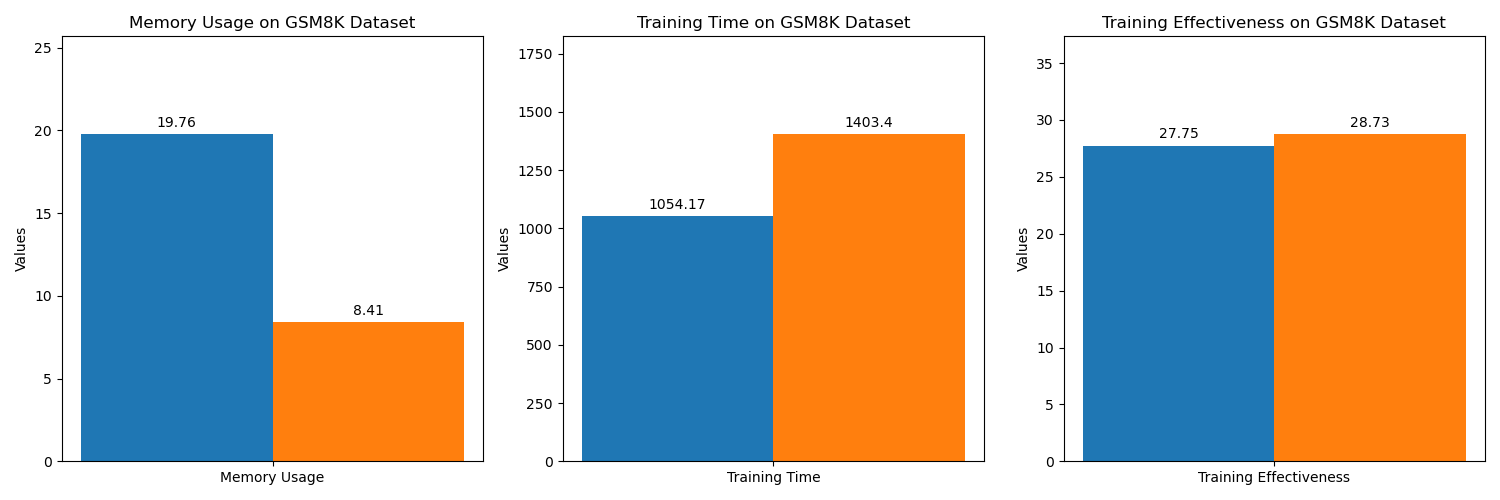
\includegraphics[width=0.5\textwidth]{GSM8K-LORA.png} % 插入图片
  \caption{基于GSM8K数据集的SFT与LoRA微调对比} % 图注
  \label{fig:my_label0} % 标签
\end{figure}
\begin{figure}[H]
  \centering
  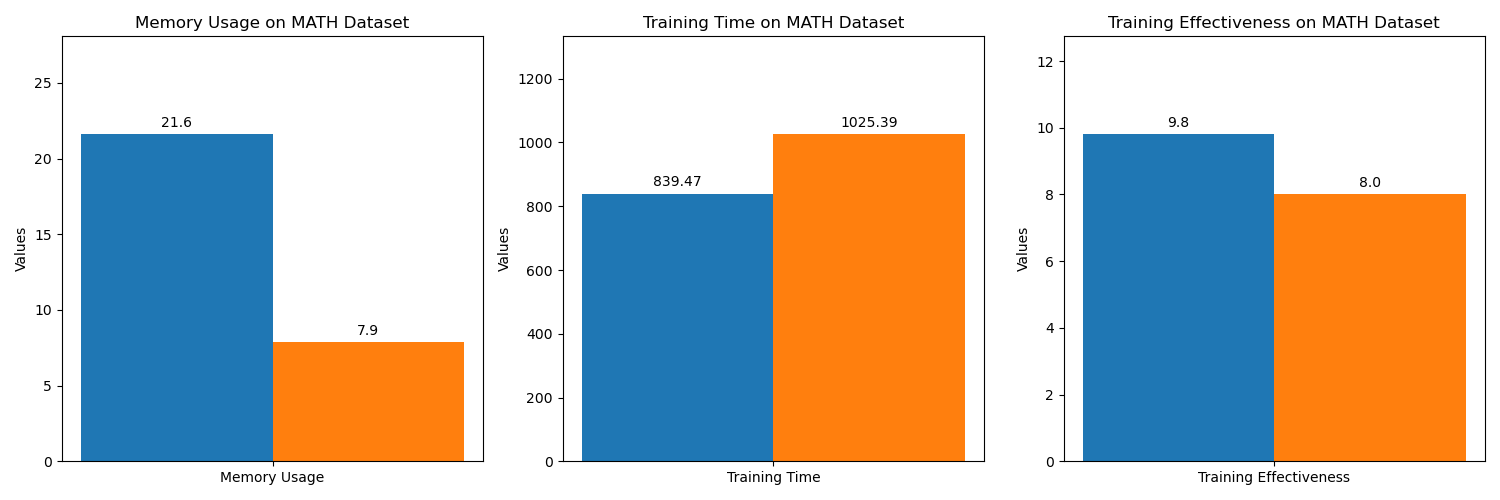
\includegraphics[width=0.5\textwidth]{MATH-LORA.png} % 插入图片
  \caption{基于MATH数据集的SFT与LoRA微调对比} % 图注
  \label{fig:my_label3} % 标签
\end{figure}

% \begin{figure}[htbp]
%   \centering
%   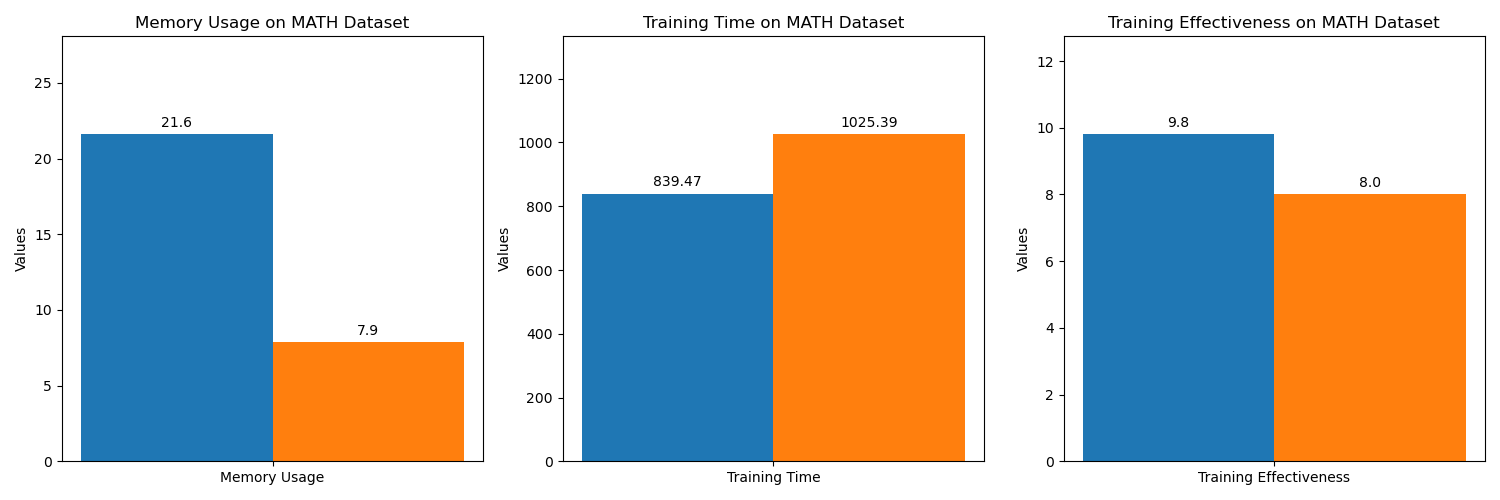
\includegraphics[width=0.5\textwidth]{MATH-LORA.png} % 插入图片
%   \caption{基于GSM8K数据集的SFT与LoRA微调对比} % 图注
%   \label{fig:my_label} % 标签
% \end{figure}
% \begin{table}[H]
%   \caption{}
%   \label{comparison-math-table}
%   \centering
%   \begin{tabular}{|c|c|c|}
%     \hline
%     \textbf{指标} & \textbf{SFT} & \textbf{LoRA} \\ \hline
%     显存占用 & 21.60GiB & 7.90GiB \\ \hline
%     训练时间 & 839.47s  & 1025.39s\\ \hline
%     训练效果 & 9.80\% &  8.00\%\\ \hline
%   \end{tabular}
% \end{table}
\textbf{分析:}
全参数微调(SFT)在训练结果上与LoRA不相上下,但由于需要更新模型的所有参数,其显存占用较高。相比之下,LoRA微调仅更新少部分适配器矩阵,显著降低了显存占用,同时在小规模任务中表现优异,且能够较好地适应不同任务。\\
但在小模型的测试上我们发现,LoRA的训练时间要长于SFT,可能原因是
\begin{itemize}
  \item 模型参数过少的影响:由于模型参数较少,全参微调的和LoRA微调的参数量相差不大,但是LoRA需要初始化以及配置其他参数。
  \item 低秩矩阵收敛较慢:LoRA通过引入低秩适配器矩阵进行微调,这可能导致梯度更新较慢,收敛时间较长。
  \item 初始优化状态差异:LoRA的低秩矩阵可能在训练初期需要更多的步骤来调整以适应任务,造成训练时间更长。
  \item 更新空间较小但复杂:尽管LoRA更新的参数较少,但低秩空间的优化可能需要更多的训练步骤来有效捕捉任务特征。
  
\end{itemize}


\subsection{基于增强数据集训练与正常训练的微调比对}
在这部分实验中,我们对比了基于增强数据集训练和正常训练的微调效果。我们对AugGSM8K和AugMATH清洗后的子数据集以及通过DeepSeek生成的扩充数据集进行了微调,并评估了训练效果。
\subsubsection{基于MuggleMath的数据增强训练}
我们基于MuggleMath数据,通过正则匹配消去重复数据,并且按一定概率采样,最后提取出两个个15k条的数据集AguGSM8K和AguMATH数据集,用于对比微调效果:
\\ Agu数据集在A10上进行训练。
\begin{table}[H]
  \caption{基于AguGSM8K训练与正常训练的微调比对}
  \label{gsm8k-augmentation-comparison-table}
  \centering
  \begin{tabular}{|c|c|c|}
    \hline
    \textbf{指标} & \textbf{正常训练} & \textbf{增强数据集训练} \\ \hline
    训练时间 & 1054.17s & 2438.16s \\ \hline
    训练效果 & 27.75\% & 42.99\% \\ \hline
  \end{tabular}
\end{table}


\begin{table}[H]
  \caption{基于AguMATH增强数据集训练与正常训练的微调比对}
  \label{math-augmentation-comparison-table}
  \centering
  \begin{tabular}{|c|c|c|}
    \hline
    \textbf{指标} & \textbf{正常训练} & \textbf{增强数据集训练} \\ \hline
    训练时间 & 839.47s & 2099.35s \\ \hline
    训练效果 & 9.80\% & 12.00\% \\ \hline
  \end{tabular}
\end{table}

\textbf{分析:}\\
结果显示,我们已经超越了基于原始数据集baseline的训练效果。
增强数据集的使用能够显著提升模型在数据多样性和鲁棒性上的表现。尽管增强数据集训练的时间较长,但其在训练效果上超越了常规训练,尤其是在数学推理等复杂任务中,增强数据集对提升模型的泛化能力具有显著作用。
\\
同时,在构造数据集的过程中,我们发现包含更多符号推导的数据集更能够增强模型的推理能力,相对于使用自然语言推导而言。
使用自然语言推导的增强数据集,反而会使得模型推理性能减弱,同时最后很难去匹配正确答案。
\subsubsection{DeepSeek生成的数据集}
我们使用DeepSeek生成的回答来扩充GSM8K和MATH训练集。DeepSeek能够生成带有详细解答步骤的回答,这种类似蒸馏的过程帮助Qwen2.5B模型提升了数学推理方面的能力。
生成的数据集包含15k条数据,但我们没有做更多处理。
\\以下在RTX 4090上进行了训练。
\begin{table}[H]
  \caption{deepseek-基于增强数据集训练与正常训练的微调比对}
  \label{deepseek-augmentation-comparison-table}
  \centering
  \begin{tabular}{|c|c|c|}
    \hline
    \textbf{指标} & \textbf{正常训练} & \textbf{增强数据集训练} \\ \hline
    训练时间 & 1054.17s & 1393.15s \\ \hline
    训练效果 & 27.75\% & 25.55\% \\ \hline
  \end{tabular}
\end{table}

\textbf{分析:}\\
这个结果表明,简单地添加更多的数据并不一定能够提升模型的表现,尤其是当这些数据是通过某种生成方式获得的时候。在机器学习和深度学习领域,数据的质量往往比数量更为重要。增强数据集需要有技巧地构造,以确保新加入的数据能够有效地补充原有数据集的不足,提供额外的信息或多样性,而不是简单地重复或引入噪声。


\subsubsection{更大模型验证}
为了验证我们的数据集的有效性和广泛适用性,我们使用3B模型进行了验证
\\ 3B模型在单张A100上进行训练
\\ 0.5B模型在单张4090上进行训练
\begin{figure}[H]
  \centering
  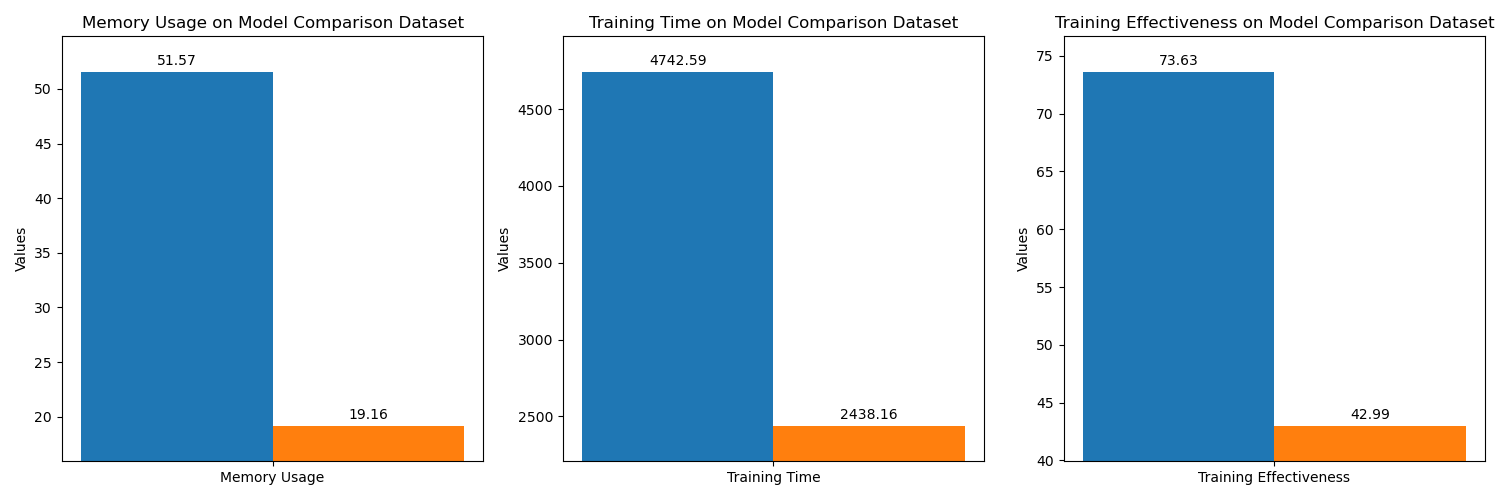
\includegraphics[width=0.5\textwidth]{scaling_graph.png} % 插入图片
  \caption{3B模型与0.5B模型的增强数据集训练对比} % 图注
  \label{fig:my_label2} % 标签
\end{figure}

\begin{figure}[H]
  \centering
  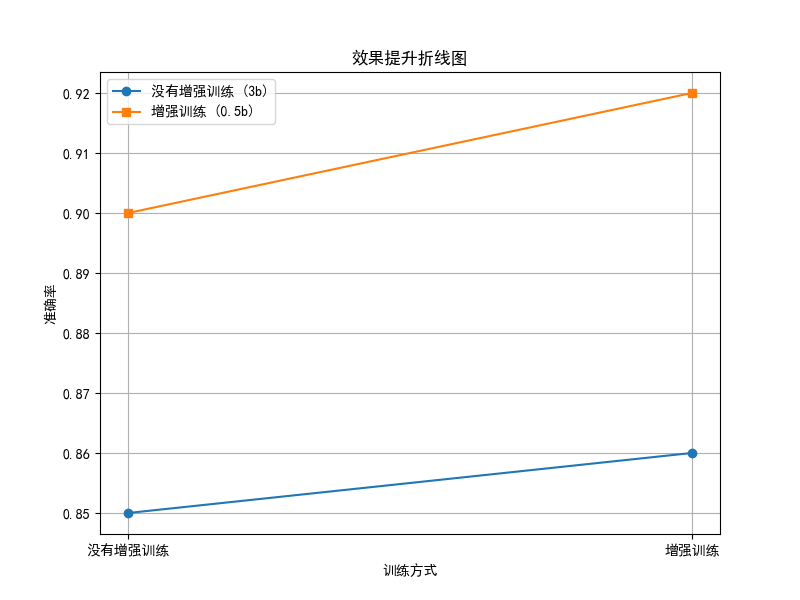
\includegraphics[width=0.5\textwidth]{compare_graph.png} % 插入图片
  \caption{效果曲线图} % 图注
  \label{fig:my_label1} % 标签
\end{figure}

\textbf{分析:}\\
通过更大模型的验证,证明了我们的增强数据集的有效性和广泛适应性。
但更大的模型提高更加有限,还是需要力大砖飞


\subsection{多轮投票机制的比对}
\\以下基于我们通过LoRA在GSM8K数据集上微调的模型进行测试。
\begin{table}[H]
  \caption{多轮投票机制的比对}
  \label{voting-mechanism-comparison}
  \centering
  \begin{tabular}{|c|c|c|c|c|}
    \hline
    \textbf{指标} & \textbf{无投票} & \textbf{一轮投票}  & \textbf{二轮投票}& \textbf{三轮投票}\\ \hline 
    训练效果 & 28.73\% & 29.69\% & 0\%& 0\% \\ \hline
  \end{tabular}
\end{table}

在多轮投票机制中,我们期望通过生成多个回答并进行投票来提升推理的鲁棒性。然而,实验结果表明,多轮投票机制并未显著提升模型的准确性,甚至在某些情况下导致训练效果下降。以下对这一现象进行详细分析:


\textbf{1. 错误答案的重复性}\\
多轮投票的基本假设是生成多个不同的答案,通过多数投票排除错误。然而,当模型生成的回答存在高度相似的错误时,投票机制无法有效纠正错误。重复的错误答案在投票中占据多数,导致最终结果仍然错误,失去了投票机制的预期优势。

\textbf{2. 模型固有偏差的影响}\\
由于模型训练数据或参数设置的固有偏差,生成的答案容易呈现出一致的错误模式。这种情况下,多轮生成并未引入足够的多样性,导致相似的错误答案被多次投票确认,进一步加剧了错误结果的稳定性。

\textbf{3. 生成结果的多样性不足}\\
多轮投票的有效性依赖于生成结果的多样性,即多个回答之间需存在一定的逻辑或内容差异。然而,实验中模型生成的回答往往高度一致,缺乏足够的多样性,使得投票机制无法剔除错误答案。此外,模型对问题的理解局限性也限制了结果的生成范围。

\textbf{4. 训练资源与优化设计限制}\\
从实验结果来看,二轮投票和三轮投票的训练效果均为 $0$,可能反映出投票机制设计与模型优化之间存在不匹配。训练过程中资源分配不均或多轮生成策略未经过有效的优化,导致投票机制无法发挥应有的作用。






  






\section{Conclusion}

本研究探索了多种方法提升Qwen系列模型在数学推理任务上的表现。\\
实验结果表明,基于全参数微调(SFT)和LoRA微调的模型在数学推理任务中表现出色,尤其是在特定任务下,通过优化计算资源能够显著提升模型的推理能力。同时,数据增强策略有效提升了模型在复杂任务中的泛化能力,尤其是在基于MuggleMath数据集清洗生成的数据集进行训练后,模型的数学推理能力得到了明显提升。
我们将两个数据集上的效果都进行了提高,在0.5B模型实验中 GSM8K 从27.75\%提升至42.99\%,MATH 从9.80\%提升至12.00\%。
然而,实验结果也表明,多轮投票机制在提高推理精度方面的效果并不显著,可能是由于生成的多个答案存在重复的错误。因此,在模型推理过程中的策略选择仍需进一步优化。此外,随着模型规模的增加,显存占用和训练时间也呈现上升趋势,如何在性能和资源消耗之间找到最佳平衡仍然是一个值得关注的研究方向。

未来的研究可以从以下几个方面进行拓展:进一步优化微调策略,探索不同类型的数据增强方法,提升多轮投票机制的鲁棒性,多步微调,PPO强化学习方法,以及探索更复杂的数学推理任务。
\section{AuthorStatement}

Huazheng Zeng : MuggleMath数据集清洗,增强数据集模型微调训练,MathSFT和Lora对比,论文Evaluation部分,论文整合\\
Yang Wang : GSM8K SFT和Lora比对 , deepseek数据集生成训练,多轮投票探索,论文Method部分\\
Yuxuan Xie :3B模型检验方法效果实验,Lora SFT对比实验,论文RelatedWord部分\\
\\其余部分由三位作者共同完成






\bibliographystyle{plainnat} % 或其他样式,如 unsrt、abbrvnat 等
\bibliography{references}    % 这里的 "references" 是你的 .bib 文件名(不含扩展名)

\end{document}